\chapter{UML Design}
\emph{UML} stands for \textbf{Unified Modeling Language} and it has been standardized by OMG\footnote{Object Management Group.}.

\paragraph{Objects}
An \emph{object} is a model of entity characterized by identity, attributes, operations it can perform and messages it can receive. The \emph{object diagram} models objects of interest in a specific case.

A \emph{link} models association between objects.

\paragraph{Classes}
A \emph{class} is a descriptor of objects with similar properties, not directly a software class, characterized by:
\begin{itemize}
\item Attributes
\begin{itemize}
\item The name of an attribute is the same for all objects and can be described in the class;
\item The value of an attribute may be different on each object and cannot described in the class.
\end{itemize}
\item Operations
\begin{itemize}
\item Are the same for all objects and can be described in the class;
\item Will be applied to different objects, possibly with different results;
\item No direct correspondence with a software function.
\end{itemize}
\end{itemize}
\textbf{An object is an instance of a class}. Each object has different values for its properties, specific for the object. In order to distinguish objects from classes, the object name is underlined.

The \emph{class diagram} models classes of interest in a specific case.

\subparagraph{Relationships}
A \emph{relationship} is a descriptor of links with similar properties characterized by its \emph{multiplicity} which identifies the maximum and the minimum number of links that can exit from an object. A relationship is always bidirectional but, at implementation level, it may not be implemented in both directions. Constraints, especially the ones involving more classes and relationships, can be expressed textually using OCL\footnote{Object Constraint Language.}.

\subparagraph{Aggregation}
\emph{B is-part-of A} means that objects described by class B can be attributes of objects described by A.

\begin{figure}[hbtp]
\centering
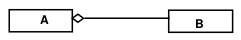
\includegraphics[scale=0.4]{images/uml_aggregation.png}
\caption{Aggregation}
\end{figure}

\subparagraph{Specialization}
\emph{A specializes B} means that objects described by A have the same properties of objects described by B, i.e.,\@ properties defined by B are inherited by A. Objects described by A can have additional properties. 

\medskip
Class diagrams are just a notation, they can be used in different documents with different goals (user requirements, developer requirements, system design).

\section{Use cases}
\emph{Uses cases} are a semi-formal notation useful to study the application domain and to identify boundaries and interactions among the system and external world. They provide a more functional view of a software system readable by customer.

Uses cases oblige the analyst to state well-defined boundaries between system and external world, organize system functions into elements on which attention is focused and supply a first basis for the specification of system structure from the user perspective.

A \textbf{scenario} is a sequence of steps describing an interaction between a user and a system. A use case is a set of scenarios tied together by a common user goal. Use case purpose is to understand how system works, while requirement purpose is to support traceability and tends to be finer grained than use case, therefore mapping is not 1:1.

\subsection{Elements}
\paragraph{Actor}
Someone or something that exchanges information with the system by supplying input to the system or by receiving output from it.

\paragraph{Use case}
A functional unit part of the system.

\paragraph{Relationships}
\emph{Relationships} follow an association models, they define which actors participate in a use case, where execution starts. Multiplicity and direction are allowed.

\subparagraph{Include}
Models that a functionality is used in the context of another functionality, i.e.,\@ one is a phase of the other.

\subparagraph{Generalization}
Defines a functionality as a specialization of another functionality (e.g.,\@ a special case). A generalization from an actor B to an actor A indicates that an instance of B can communicate with the same kinds of use-case instances as an instance of A.

\subparagraph{Extension}
An extended relationship from use case A to use case B indicates that an instance of use case B may be augmented by the behavior specified by A. The behavior is inserted at the location defined by the extension point in B, which is referenced by the extend relationship.

\paragraph{Use case and class diagrams}
They must be consistent:
\begin{itemize}
\item An actor may become a class;
\item A use case must become one operation on a class and may originate several operations on several classes;
\item Interaction are not represented.
\end{itemize}